%%%%%%%%%%%%%%%%%%%%%%%%%%%%%%%%%%%%%%%%%%%%%%%%%%%%%%%%%%%%%%%%%%%%%%%%%%%%%%%
\section{Potential Solutions}
\label{sec:solutions}
%%%%%%%%%%%%%%%%%%%%%%%%%%%%%%%%%%%%%%%%%%%%%%%%%%%%%%%%%%%%%%%%%%%%%%%%%%%%%%%

first paragraph: outline following sections
-recall issues from before
   -over-prediction of U-238 capture in resonance groups results in a non-negligible eigenvalue bias
-~\autoref{subsec:angular-mgxs} intros fully angular-dependent MGXS in the context of the first test case
-~\autoref{subsec:sph} intros SPH factors in the context of the second test case


%%%%%%%%%%%%%%%%%%%%%%%%%%%%%%%%%%%%%%%%%%%%%%%%%%%%%%%%%%%%%%%%%%%%%%%%%%%%%%%
\subsection{Angularly-Dependent Total MGXS}
\label{subsec:angular-mgxs}

The flux separability approximation introduced in~\autoref{sec:flux-separability} led to the use of the scalar rather than the angular flux to condense the total cross section in energy. The mathematically proper treatment would instead use the angular flux to condense the total MGXS in angle, energy and space, resulting in angularly-dependent total MGXS. This section shows that using fully angularly-dependent data causes the bias in the group reaction rates to vanish for the first test case benchmark.

As was noted in~\autoref{sec:flux-separability}, the most important aspect of the physics to account for in an LWR fuel pin is whether neutrons are entering the region through the fuel pin or directly from the moderator (see~\autoref{fig:incoming-outgoing}). This self-shielding effect cannot be properly modeled by the simple application of angularly-dependent to a single region fuel pin. In this case, a cross section for a given angle would be applied to both neutrons entering the fuel pin from the moderator and to neutrons exiting the fuel pin on the opposite side. Thus, the fuel pin must also be spatially-discretized in order to resolve the error.

The impact of angularly-dependent MGXS was investigated for first test case benchmark of a simple two-region pin cell. The reference solution was computed on an ultra-fine energy mesh and was used to collapse cross sections. Cross sections for the left hand side of the transport equation were collapsed separately for each angle, weighted by the angular flux for that angle. The geometry was discretized with eight equally-spaced azimuthal sectors. The fuel was split up into three rings of equal volume, while the moderator was subdivided into two equal width rings. {\color{red} How many ultra-fine energy groups? How many discrete angular bins? Include all information necessary to reproduce these results.}

The reaction rate errors in resonance groups with angular flux-weighted MGXS are presented in~\autoref{tab:angular-mgxs-case1}. The results for scalar flux-weighted MGXS given in~\autoref{tab:case1-bias} are reproduced here for clarity. The most significant errors in energy groups 24, 25 and 27 are reduced by up to two orders of magnitude with angularly-dependent MGXS. These results demonstrate that the observed condensation errors can be removed by maintaining fine structure in both angle and space in the condensed cross sections.

\begin{table}[h!]
  \centering
  \caption{U-238 resonance range reaction rate percent relative errors computed with scalar and angular flux-weighted MGXS for the first test case benchmark {(\color{red}Table 7.5 from Nate's thesis)}.}
  \label{tab:angular-mgxs-case1}
  \begin{tabular}{c c c c c}
  \toprule
  & & \multicolumn{2}{c}{Error [\%]} \\
  \cline{3-4}
  Group & $E_{max}$ [eV] & Scalar & Angular \\
  \midrule
  15 & 9118.00 & 1.29E-01 & 9.93E-03 \\
  16 & 5530.00 & 1.75E-01 & 1.23E-02 \\
  17 & 3519.10 & 4.04E-01 & 2.68E-02 \\
  18 & 2239.45 & 5.67E-01 & 3.70E-02 \\
  19 & 1425.10 & 5.75E-01 & 3.64E-02 \\
  20 & 906.899 & 3.65E-01 & 2.20E-02 \\
  21 & 367.263 & 6.99E-01 & 4.87E-02 \\
  22 & 148.729 & 7.75E-01 & 5.78E-02 \\
  23 & 75.5014 & 6.47E-01 & 4.90E-02 \\
  24 & 48.0520 & 1.24E+00 & 1.10E-02 \\
  25 & 27.7000 & 1.27E+00 & 1.18E-02 \\
  26 & 15.9680 & 1.29E-03 & 3.45E-02 \\
  27 & 9.87700 & 1.34E+00 & 1.21E-01 \\
  \bottomrule
\end{tabular}
\end{table}

Although this demonstration fully diagnoses the observed errors, this does not suggest that the ultimate solution to condensation errors is to use such fine structure. This would come at a great computational expense, as the spatial discretization increases the cost of the transport solve, and the angularly-dependent cross sections dramatically increase the memory requirements. In addition, flux separability is commonly used since conventional MGXS generation schemes are generally incapable of approximating the angular dependence of the flux in the arbitrary geometries and spatial discretizations modeled by multi-group transport codes.

%As a result, multi-group codes are unable to reproduce the correct angular dependence of the neutron flux with scalar flux-weighted MGXS. Furthermore, flux separability is an approximation which may lead to non-trivial errors in downstream multi-group calculations, such as the eigenvalue bias observed in~\autoref{sec:test-case2}.

%%%%%%%%%%%%%%%%%%%%%%%%%%%%%%%%%%%%%%%%%%%%%%%%%%%%%%%%%%%%%%%%%%%%%%%%%%%%%%%
\subsection{SuPerHomog\'{e}n\'{e}isation Factors}
\label{subsec:sph}

Hmm \cite{hebert2005ribon}, \cite{hebert1993consistent} \cite{hebert1997advances}

Although angularly-dependent total MGXS the most direct solution to eliminate the flux separability approximation, it is not a desirable approach for a number of reasons. Angularly-dependent MGXS would significantly increase the memory footprint for MGXS libraries, and be complicated to accommodate in multi-group methods. SuPerHomog\'{e}n\'{e}isation (SPH) factors is presented in this section as an alternative method to reduce heterogeneous resonant reaction rate errors. SPH is a relatively simple-to-implement method, which was evaluated in OpenMOC as discussed in the following sections.


%%%%%%%%%%%%%%%%%%%%%%%%%%%%%%%%%%%%%%%%%%%%%%%%%%%%%%%%%%%%%%%%%%%%%%%%%%%%%%%
\subsubsection{Overview}
\label{subsubsec:sph-overview}

The SPH algorithm enforces reaction rate preservation between a reference fine-mesh transport problem and a corresponding coarse mesh transport or diffusion problem in energy and space. SPH factors have traditionally been applied to spatially-homogenized few-group MGXS for coarse mesh diffusion applications. However, this section will introduce SPH factors to enforce equivalence between continuous energy Monte Carlo and deterministic multi-group transport methods. 

The SPH scheme postulates the existence of a set of factors $\mu_{k,g}$ for each spatial zone $k$ and energy group $g$ which force the streaming and collision terms in the transport equation to balance with a fixed source $Q_{k,g}$:

\begin{dmath}
\label{eqn:sph-transport-eqn}
\mathbf{\Omega} \cdot \nabla \psi_{g}(\mathbf{r},\mathbf{\Omega}) + \mu_{k,g}\Sigma_{t,k,g}\psi_{g}(\mathbf{r},\mathbf{\Omega}) = Q_{k,g}(\mathbf{\Omega})
\end{dmath}

\noindent In this equation, the SPH factors are applied to correct the total MGXS in each region and group. The fixed source $Q_{k,g}$ is computed from the reference fine-mesh solution. In this case, the fixed source is treated as the sum of scattering and fission production sources in each energy group and spatial zone. For example, continuous energy Monte Carlo can be used to compute reference multi-group fluxes and MGXS, which are then combined to compute an isotropic source as follows:

\begin{dmath}
\label{eqn:sph-source}
Q_{k,g}(\mathbf{\Omega}) = \frac{1}{4\pi} \sum_{g'=1}^{G} \Sigma_{s,k,g' \rightarrow g}\phi_{k,g'} + \frac{\chi_{k,g}}{4\pi k_{eff}}\sum_{g'=1}^{G} \nu\Sigma_{f,k,g'}\phi_{k,g'}
\end{dmath}

\noindent Given the fixed source and total MGXS from MC,~\autoref{eqn:sph-transport-eqn} may be solved using any multi-group transport method, such as MOC. The challenge is to devise estimates to the true SPH factors $\mu_{k,g}$ which adequately preserve reaction rates. The following section describes the iterative scheme used to estimate SPH factors.


%%%%%%%%%%%%%%%%%%%%%%%%%%%%%%%%%%%%%%%%%%%%%%%%%%%%%%%%%%%%%%%%%%%%%%%%%%%%%%%
\subsubsection{Algorithm}
\label{subsubsec:sph-algorithm}

An iterative algorithm is used to estimate SPH factors from a series of multi-group fixed source calculations. First, the estimates $\mu_{k,g}^{(n)}$ at iteration $n$ to the true SPH factors $\mu_{k,g}$ are introduced as a correction factor for the total cross section in~\autoref{eqn:sph-transport-eqn}:

\begin{dmath}
\label{eqn:sph-transport-eqn-iterate}
\mathbf{\Omega} \cdot \nabla \psi_{g}^{(n)}(\mathbf{r},\mathbf{\Omega}) + \mu_{k,g}^{(n-1)}\Sigma_{t,k,g}\psi_{g}^{(n)}(\mathbf{r},\mathbf{\Omega}) = Q_{k,g}(\mathbf{\Omega})
\end{dmath}

\noindent A multi-group transport code (such as OpenMOC) may be used to solve~\autoref{eqn:sph-transport-eqn-iterate} with angular and volume integration to compute the scalar flux distribution. The SPH factor estimates $\mu_{k,g}^{(n)}$ are found from the ratio of the reference Monte Carlo scalar flux $\phi_{k,g}^{MC}$ to the flux $\phi_{k,g}^{(n)}$ computed from the fixed source calculation at iteration $n$,

\begin{equation}
\label{eqn:sph-update}
\mu_{k,g}^{(n)} = \frac{\phi_{k,g}^{MC}}{\phi_{k,g}^{(n)}}
\end{equation}

\noindent where the factors are initialized to unity on the first iteration. The SPH factors are used to find a total MGXS which forces neutron balance in~\autoref{eqn:sph-transport-eqn-iterate}. The initial total MGXS $\Sigma_{t,k,g}^{(0)}$ is computed from the reference MC flux and total reaction rate tallies. The SPH factors are then used to obtain a corrected total MGXS $\Sigma_{t,k,g}^{(n)}$ on each iteration:

\begin{dmath}
\label{eqn:sph-update-sigt}
\Sigma_{t,k,g}^{(n)} = \mu_{k,g}^{(n-1)}\Sigma_{t,k,g}^{(0)}
\end{dmath}

The series of fixed source problems defined by~\autoref{eqn:sph-transport-eqn-iterate} are solved until the SPH factors converge.

The scattering matrix $\Sigma_{s,k,g'\rightarrow g}$ and fission production cross section $\nu\Sigma_{f,k,g}$ are used to compute the reference fixed source in~\autoref{eqn:sph-source}, but are not needed in the iterative scheme defined in Eqn.~\ref{eqn:sph-transport-eqn-iterate}. However, in the context of this thesis, SPH factors are computed to preserve reaction rates in subsequent eigenvalue calculations. Therefore, the SPH factors must be applied to the scattering matrix and fission production cross sections to produce a fully-corrected MGXS library.

The SPH iteration algorithm described here is summarized in~\autoref{alg:sph}. It should be noted that as presently posed, there is no unique solution to the set of SPH factors which preserve reaction rates. A unique solution may be found by forcing the factors to be unity in non-fissile zones (\textit{e.g.}, moderator, clad and gap). This approach is motivated by the fact that resonances which lead to self-shielding errors -- such as the U-238 capture resonances -- are generally from isotopes in the fuel. However, the reaction rates in non-fissile zones will not be preserved since the MGXS in these zones remain uncorrected, but these errors are likely dominated by those in the fuel as was shown previously.

\begin{algorithm}[h]
\caption{SPH Factor Algorithm}
\label{alg:sph}
\begin{algorithmic}[1]
  \State Initialize MGXS from MC tallies
  \State Compute reference source from MC flux and MGXS
  \State Initialize SPH factors to unity
  \While{SPH factors are not converged}
    \State Update total MGXS with SPH factors
    \State Solve fixed source transport problem\footnotemark
    \State Compute new SPH factors
  \EndWhile
  \State Update all MGXS with SPH factors
\end{algorithmic}
\end{algorithm}

\footnotetext{A series of $G$ independent fixed source problems may be solved for each of the $G$ groups. Alternatively, a single fixed source problem may simultaneously solve for all $G$ groups, as is done in OpenMOC.}


%%%%%%%%%%%%%%%%%%%%%%%%%%%%%%%%%%%%%%%%%%%%%%%%%%%%%%%%%%%%%%%%%%%%%%%%%%%%%%%
\subsection{Results}
\label{sec:sph-results}

\begin{figure}[h!]
\centering
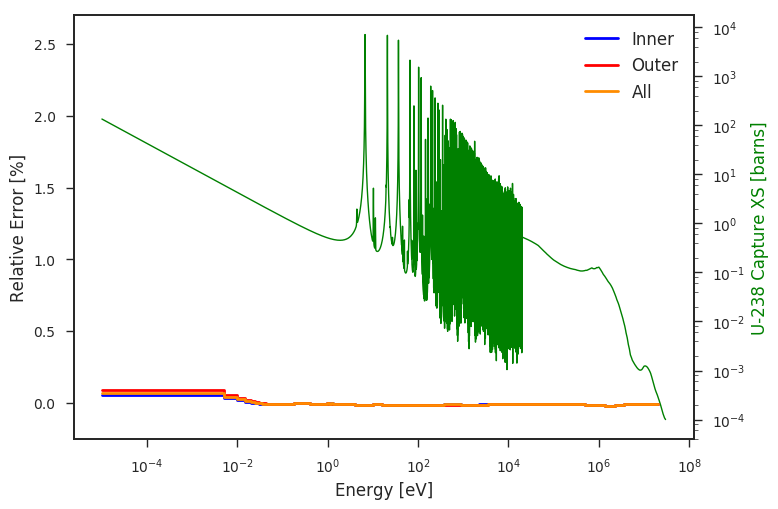
\includegraphics[width=\linewidth]{figures/rel-err-inner-outer-sph}
\caption{The energy-dependent relative error of the OpenMOC scalar flux computed with SPH-corrected MGXS with respect to the reference OpenMC flux for the innermost, outermost and all FSRs.}
\label{fig:rel-err-energy-sph}
\end{figure}

\begin{table}[h!]
  \centering
  \caption{The eigenvalue bias with SPH-corrected MGXS.}
  \label{table:keff-bias-sph} 
  \begin{tabular}{c S[table-format=6.1] S[table-format=6.1] S[table-format=6.1]}
  \toprule
  & \multicolumn{3}{c}{{\bf FSR Discretization}} \\
  \midrule
  \multicolumn{1}{c}{{\bf \# Groups}} &
  {\bf 1$\times$} & {\bf 4$\times$} & {\bf 16$\times$} \\
  \midrule
1 & 19 & -18 & -14 \\
2 & 25 & -14 & -6 \\
4 & 7 & 2 & 1 \\
8 & 4 & -0 & 2 \\
16 & 5 & 0 & 4 \\
25 & 5 & 2 & -1 \\
40 & 4 & 3 & -2 \\
70 & 4 & 2 & -3 \\
  \bottomrule
\end{tabular}
\end{table}